% last updated in April 2002 by Antje Endemann
% Based on CVPR 07 and LNCS, with modifications by DAF, AZ and elle, 2008 and AA, 2010, and CC, 2011; TT, 2014; AAS, 2016

\documentclass[runningheads]{llncs}
\usepackage{graphicx}
\usepackage{caption}

\usepackage{amsmath,amssymb} % define this before the line numbering.
\usepackage{ruler}
\usepackage{color}
\usepackage{array}
\usepackage{cite}

\captionsetup[table]{skip=3pt}

\newcommand{\etal}{\mbox{\emph{et al.\ }}}

\usepackage[width=122mm,left=12mm,paperwidth=146mm,height=193mm,top=12mm,paperheight=217mm]{geometry}

\makeatletter
\newcommand{\thickhline}{%
    \noalign {\ifnum 0=`}\fi \hrule height 1pt
    \futurelet \reserved@a \@xhline
}

\makeatletter
\renewcommand\paragraph{\@startsection{paragraph}{4}{\z@}%
           {1.25ex \@plus1ex \@minus.2ex}%
           {-1em}%
           {\normalfont\normalsize\bfseries}}
            
\renewcommand\subsubsection{\@startsection{subsubsection}{3}{\z@}%
                {-2ex\@plus -1ex \@minus -.2ex}%
                {0.1ex \@plus .2ex}%
                {\normalfont\normalsize\bfseries}}
                
                
\newcolumntype{"}{@{\hskip\tabcolsep\vrule width 1pt\hskip\tabcolsep}}
\makeatother

\begin{document}
% \renewcommand\thelinenumber{\color[rgb]{0.2,0.5,0.8}\normalfont\sffamily\scriptsize\arabic{linenumber}\color[rgb]{0,0,0}}
% \renewcommand\makeLineNumber {\hss\thelinenumber\ \hspace{6mm} \rlap{\hskip\textwidth\ \hspace{6.5mm}\thelinenumber}}
% \linenumbers
\pagestyle{headings}
\mainmatter
\def\ECCV16SubNumber{1644}  % Insert your submission number here

\title{Joint Event Recognition and Image Curation \\ (Supplementary Material)} % Replace with your title

\titlerunning{ECCV-16 submission ID \ECCV16SubNumber}

\authorrunning{ECCV-16 submission ID \ECCV16SubNumber}

\author{Anonymous ECCV submission}
\institute{Paper ID \ECCV16SubNumber}


\maketitle
\section{Performance - Iteration number}
In the main paper, we described the iterative curation-recognition procedure which iteratively updates album-wise event type prediction and image-wise importance score prediction. In case the procedure does not converge and oscillates, the final event type / image importance prediction is averaged over last 3 iterations. There are two hyperparameters for the iterative procedure: $\theta = (m, \alpha)$. Here, $m$ is the threshold for the minimum fraction of the maximum probability to consider, which eliminates the event types with low confidence for image importance prediction; $\alpha$ is the emphasis we put on the image importance score for event type prediction.

 The hyperparameters are decided with a validation set. In this section, we analyze the algorithm performance with respect to the iteration number on ML-CUFED Dataset.

\subsection{Event Recognition Performance - Iteration Number }
\label{recognition_section}
There is more than one possible choice for $\theta$ from the event recognition result of validation set, and if we look into the trend of the recognition accuracy over the iteration number, there are several different types, as shown in Figure~\ref{recognition_iterall}. To show the different trends more clearly, Figure~\ref{recognition_iter} illustrates individual plot for different $\theta$.

We can see that it takes different steps to converge for different choices of $\theta$. For Figure~\ref{recognition_iter}(a), $m = 0.9$, and this means only event types with very high prediction confidence are considered to contribute to the image importance prediction. It takes only two steps to converge. In contrast, for Figure~\ref{recognition_iter}(c), $m=0.1$, and this means that more events can contribute to the importance prediction. This results in the slower changes of image importance score prediction and  event type prediction over iterations, and as shown in Figure~\ref{recognition_iter}(c), it takes 5 iterations to converge. For Figure~\ref{recognition_iter}(b), $m=0.3$, and it takes 3 iterations to converge, which is in the middle of Figure~\ref{recognition_iter}(a) and (c).

Figure~\ref{recognition_iter}(d) also shows the case where the iterative algorithm does not converge, and the last recognition result is produced by averaging the final 3 iterations.


\begin{figure}
\vspace{-0.1in}
\centering
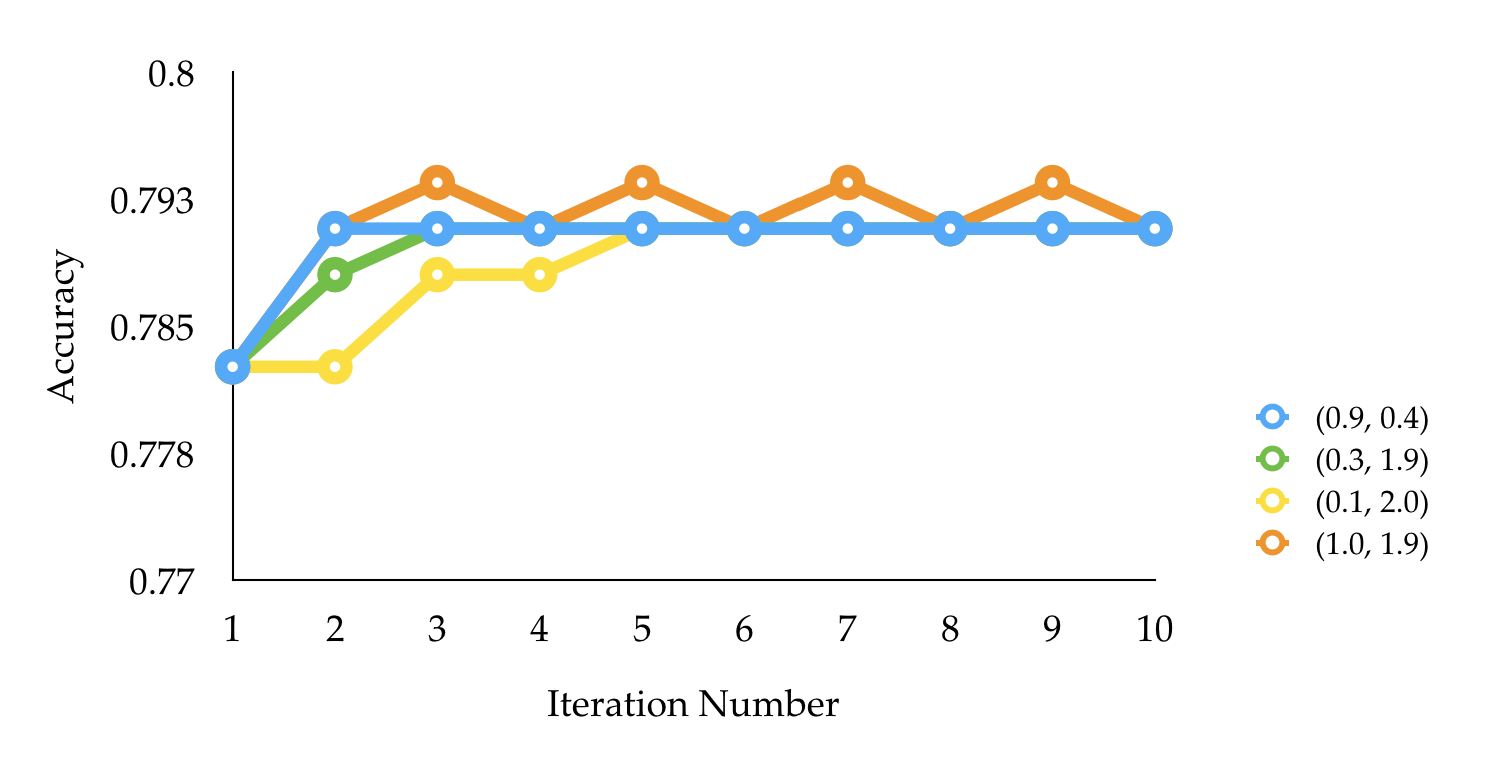
\includegraphics[width=4in]{recognition_iterall}
\caption{Album-wise event recognition accuracy v.s. iteration number for four different choices of hyperparameters $ (m, \alpha)$ of the iterative curation-recognition procedure.}
\label{recognition_iterall}
\vspace{-0.2in}
\end{figure}

\begin{figure}
\vspace{-0.1in}
\centering
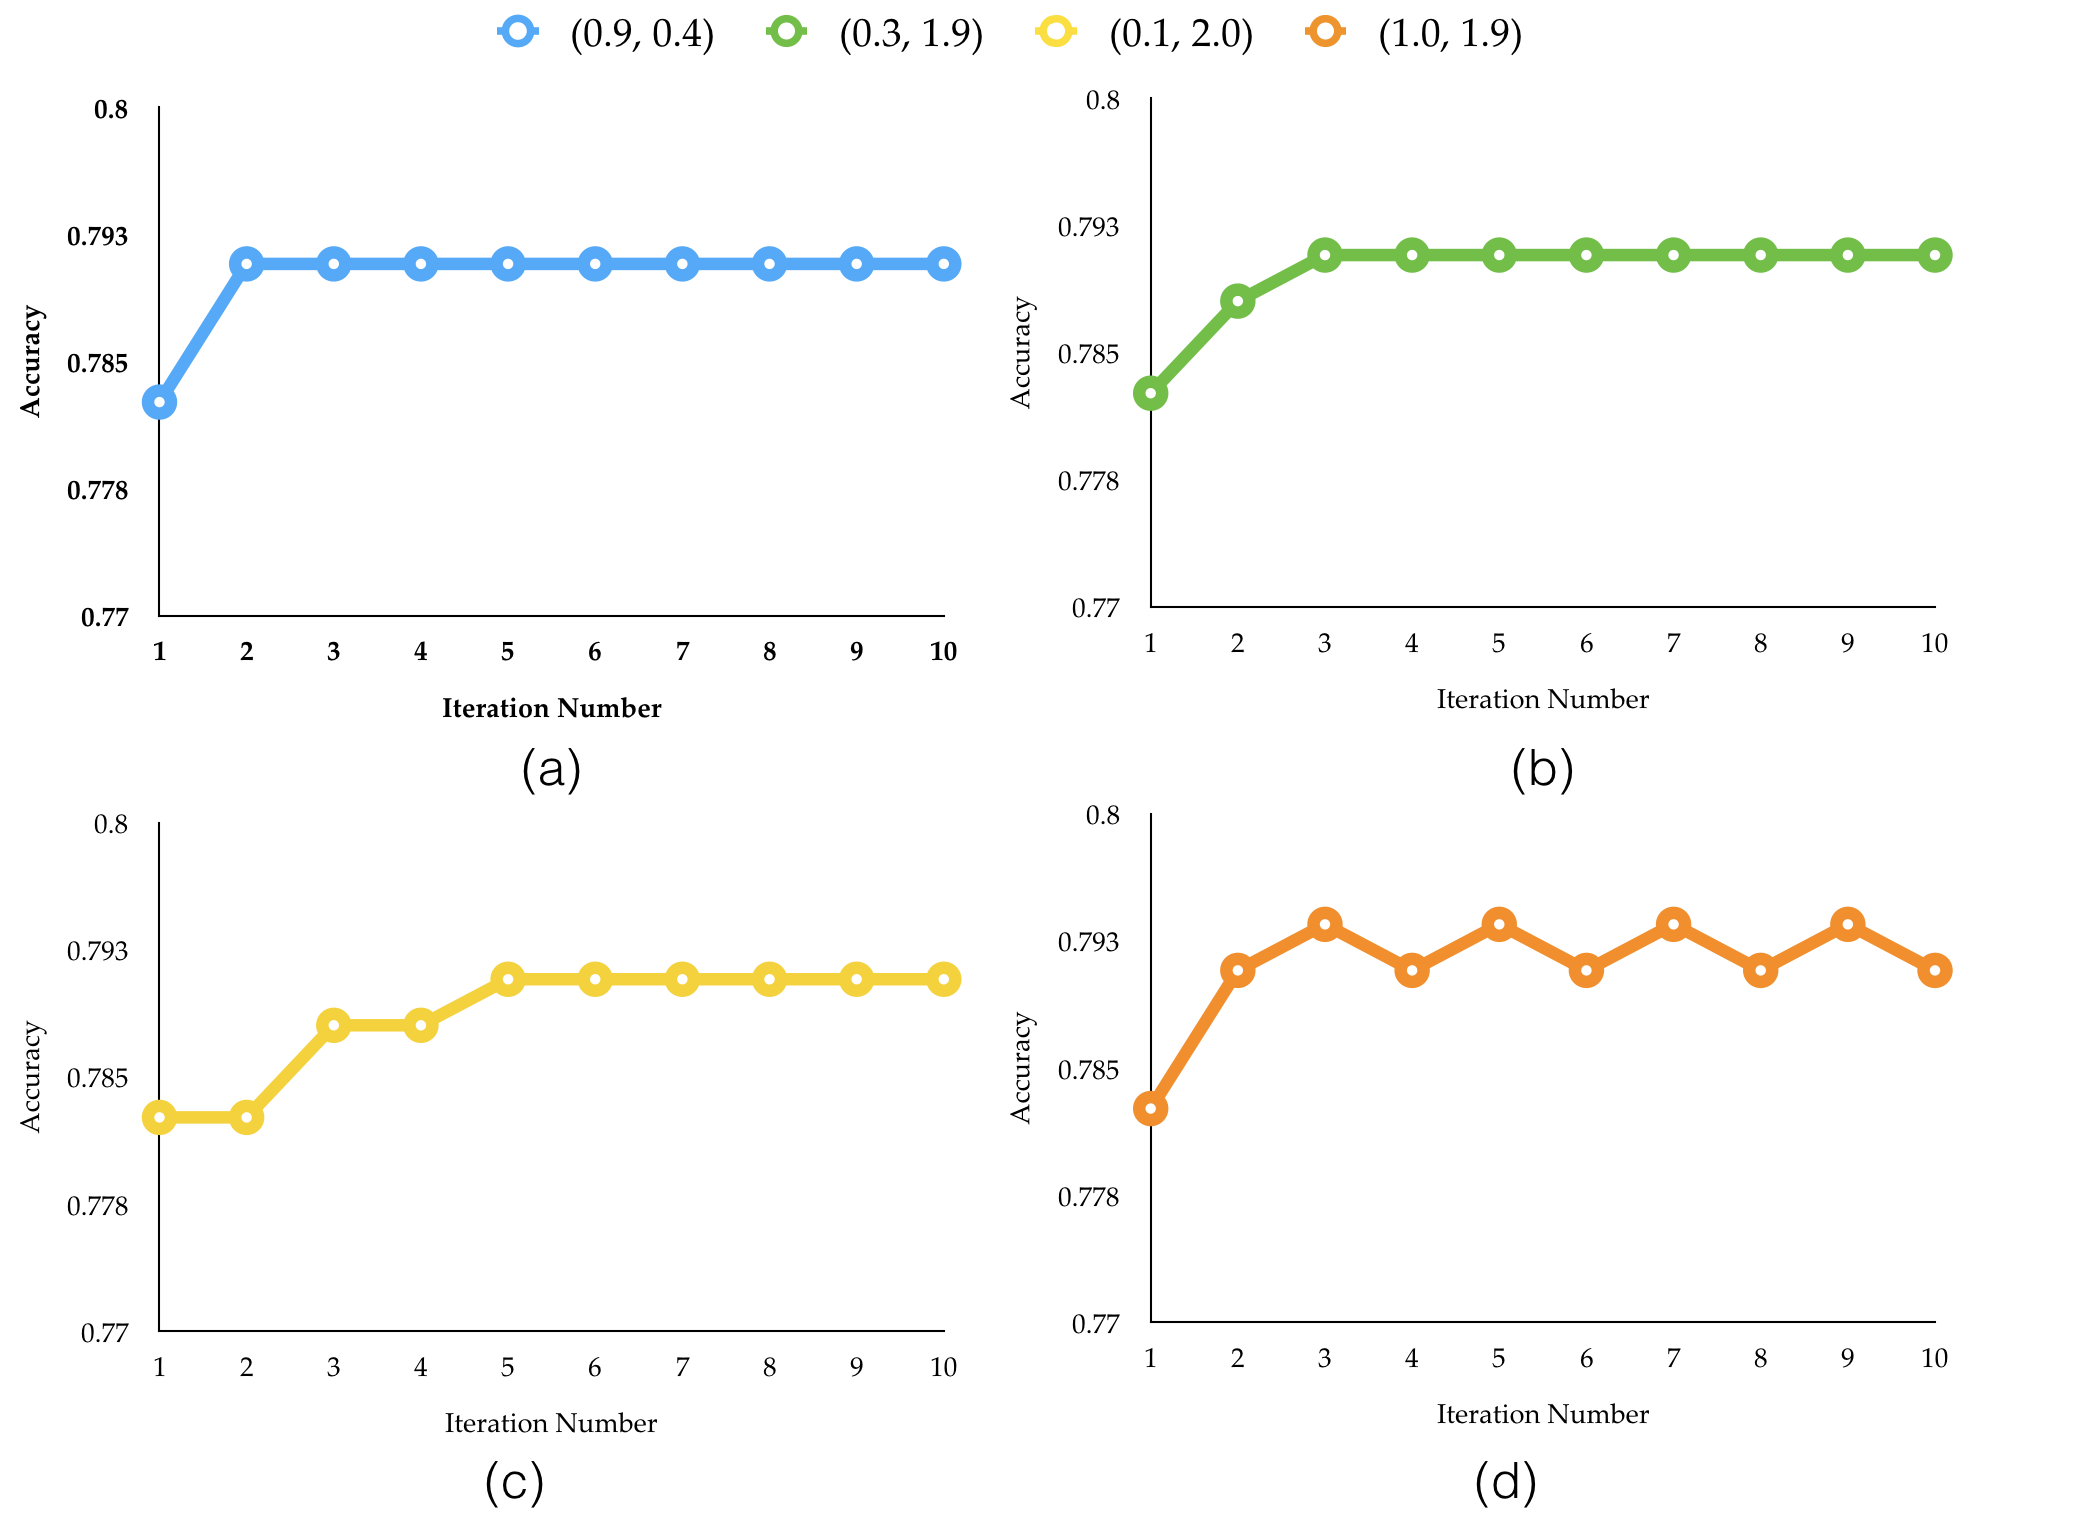
\includegraphics[width=4.8in]{recognition_iter}
\caption{ (Separately shown) Album-wise event recognition accuracy v.s. iteration number for four different choices of hyperparameters $ (m, \alpha)$ of the iterative curation-recognition procedure.}
\label{recognition_iter}
\vspace{-0.2in}
\end{figure}

\subsection{Image Importance Prediction Performance - Iteration Number }
Starting from the possible choices of $\theta$ we get in Section~\ref{recognition_section}, we can further filter the choice with the image importance prediction result on the validation set. The image importance score performance (measured by MAP@$10\%$ with iteration number) for the final choice of $\theta$ is shown in Figure~\ref{importance_iter}. Note that the iterative updating algorithm is initialized with equal image importance score for every image. Therefore, first iteration importance score is calculated from the event recognition result with 78.2\% accuracy, while first iteration event recognition is calculated from equal importance score, which is  obviously not a good image score prediction. Therefore, we expect a greater gain after iterative updates for event recognition than image importance prediction. As shown, the performance converges after second iteration.

\begin{figure}
\vspace{-0.1in}
\centering
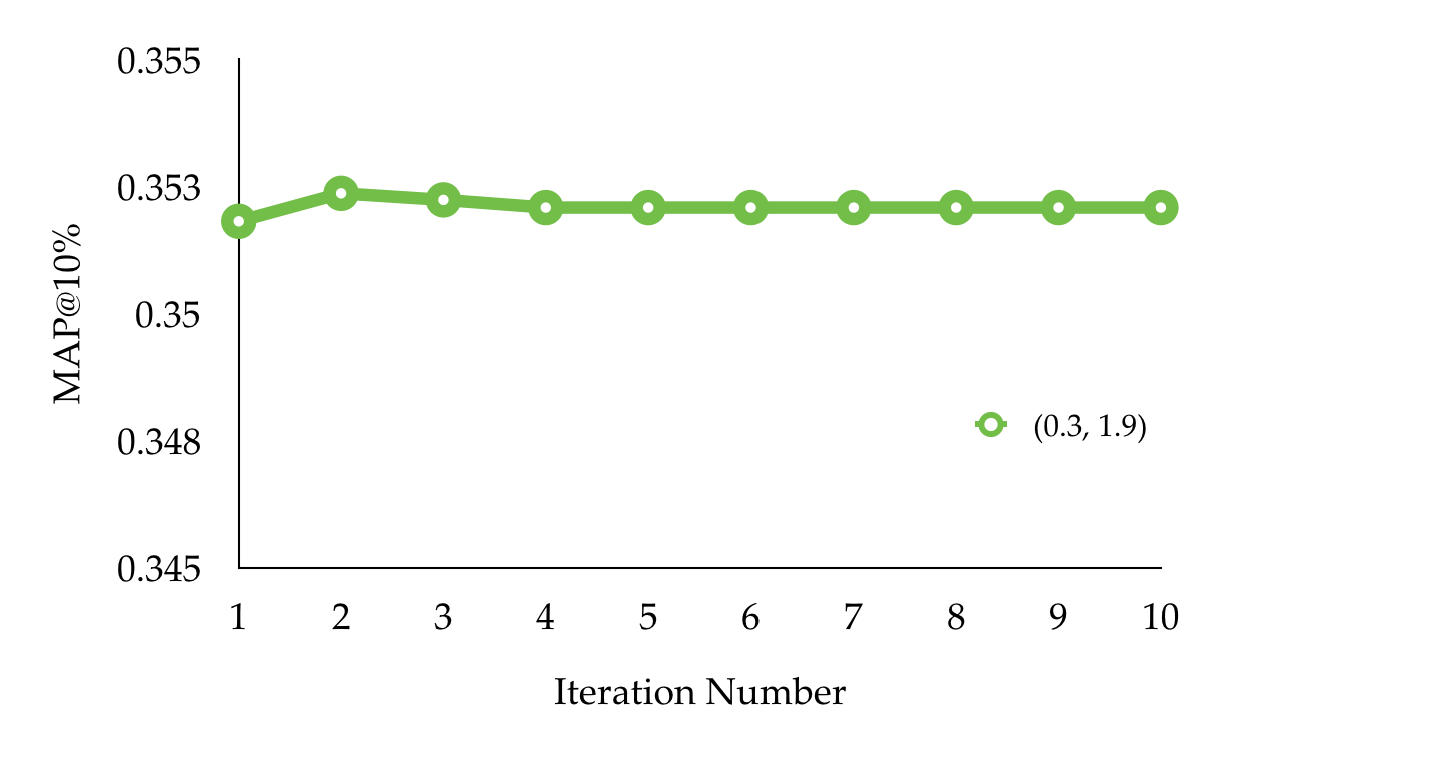
\includegraphics[width=4in]{importance_iter}
\caption{For final choice of $\theta=(m, \alpha) = (0.3, 1.9)$, the image importance prediction accuracy v.s. iteration number.}
\label{importance_iter}
\vspace{-0.2in}
\end{figure}

\section{Qualitative results}
In this section, we show more examples of the qualitative result from our algorithm.

In Figure~\ref{correct1}, four albums in ML-CUFED Dataset are shown. For the examples shown here, the album-wise event type prediction is wrong with CNN-recognition method (with only a CNN to predict event type of single images, and averaging the prediction from every image in an album for final prediction), but with the proposed CNN-LSTM-Iterative algorithm, the event type prediction is correct. Also, we can see the ground-truth and predicted importance ranking of the images in each album. Only a fraction of images in the albums are shown here due to limited space. We deliberately choose both images with high ground-truth importance and low ground-truth importance for each album to show the overall quality of the albums.

In the first example of a Cruise Trip album, there are many images of the iceberg and the sea like the last image shown here. If only CNN-recognition is used, and the prediction is produced by averaging the prediction of every image in the album, and the album is recognized as Beach Trip. However, after we assign different importance score to images, as shown the ranking of images, this album is correctly recognized as Cruise Trip. This indicates the advantage of the joint recognition-curation algorithm. In other words, our full method is able to rank important images (which are more indicative of event types) on the top. 
 
\begin{figure}
\vspace{-0.1in}
\centering
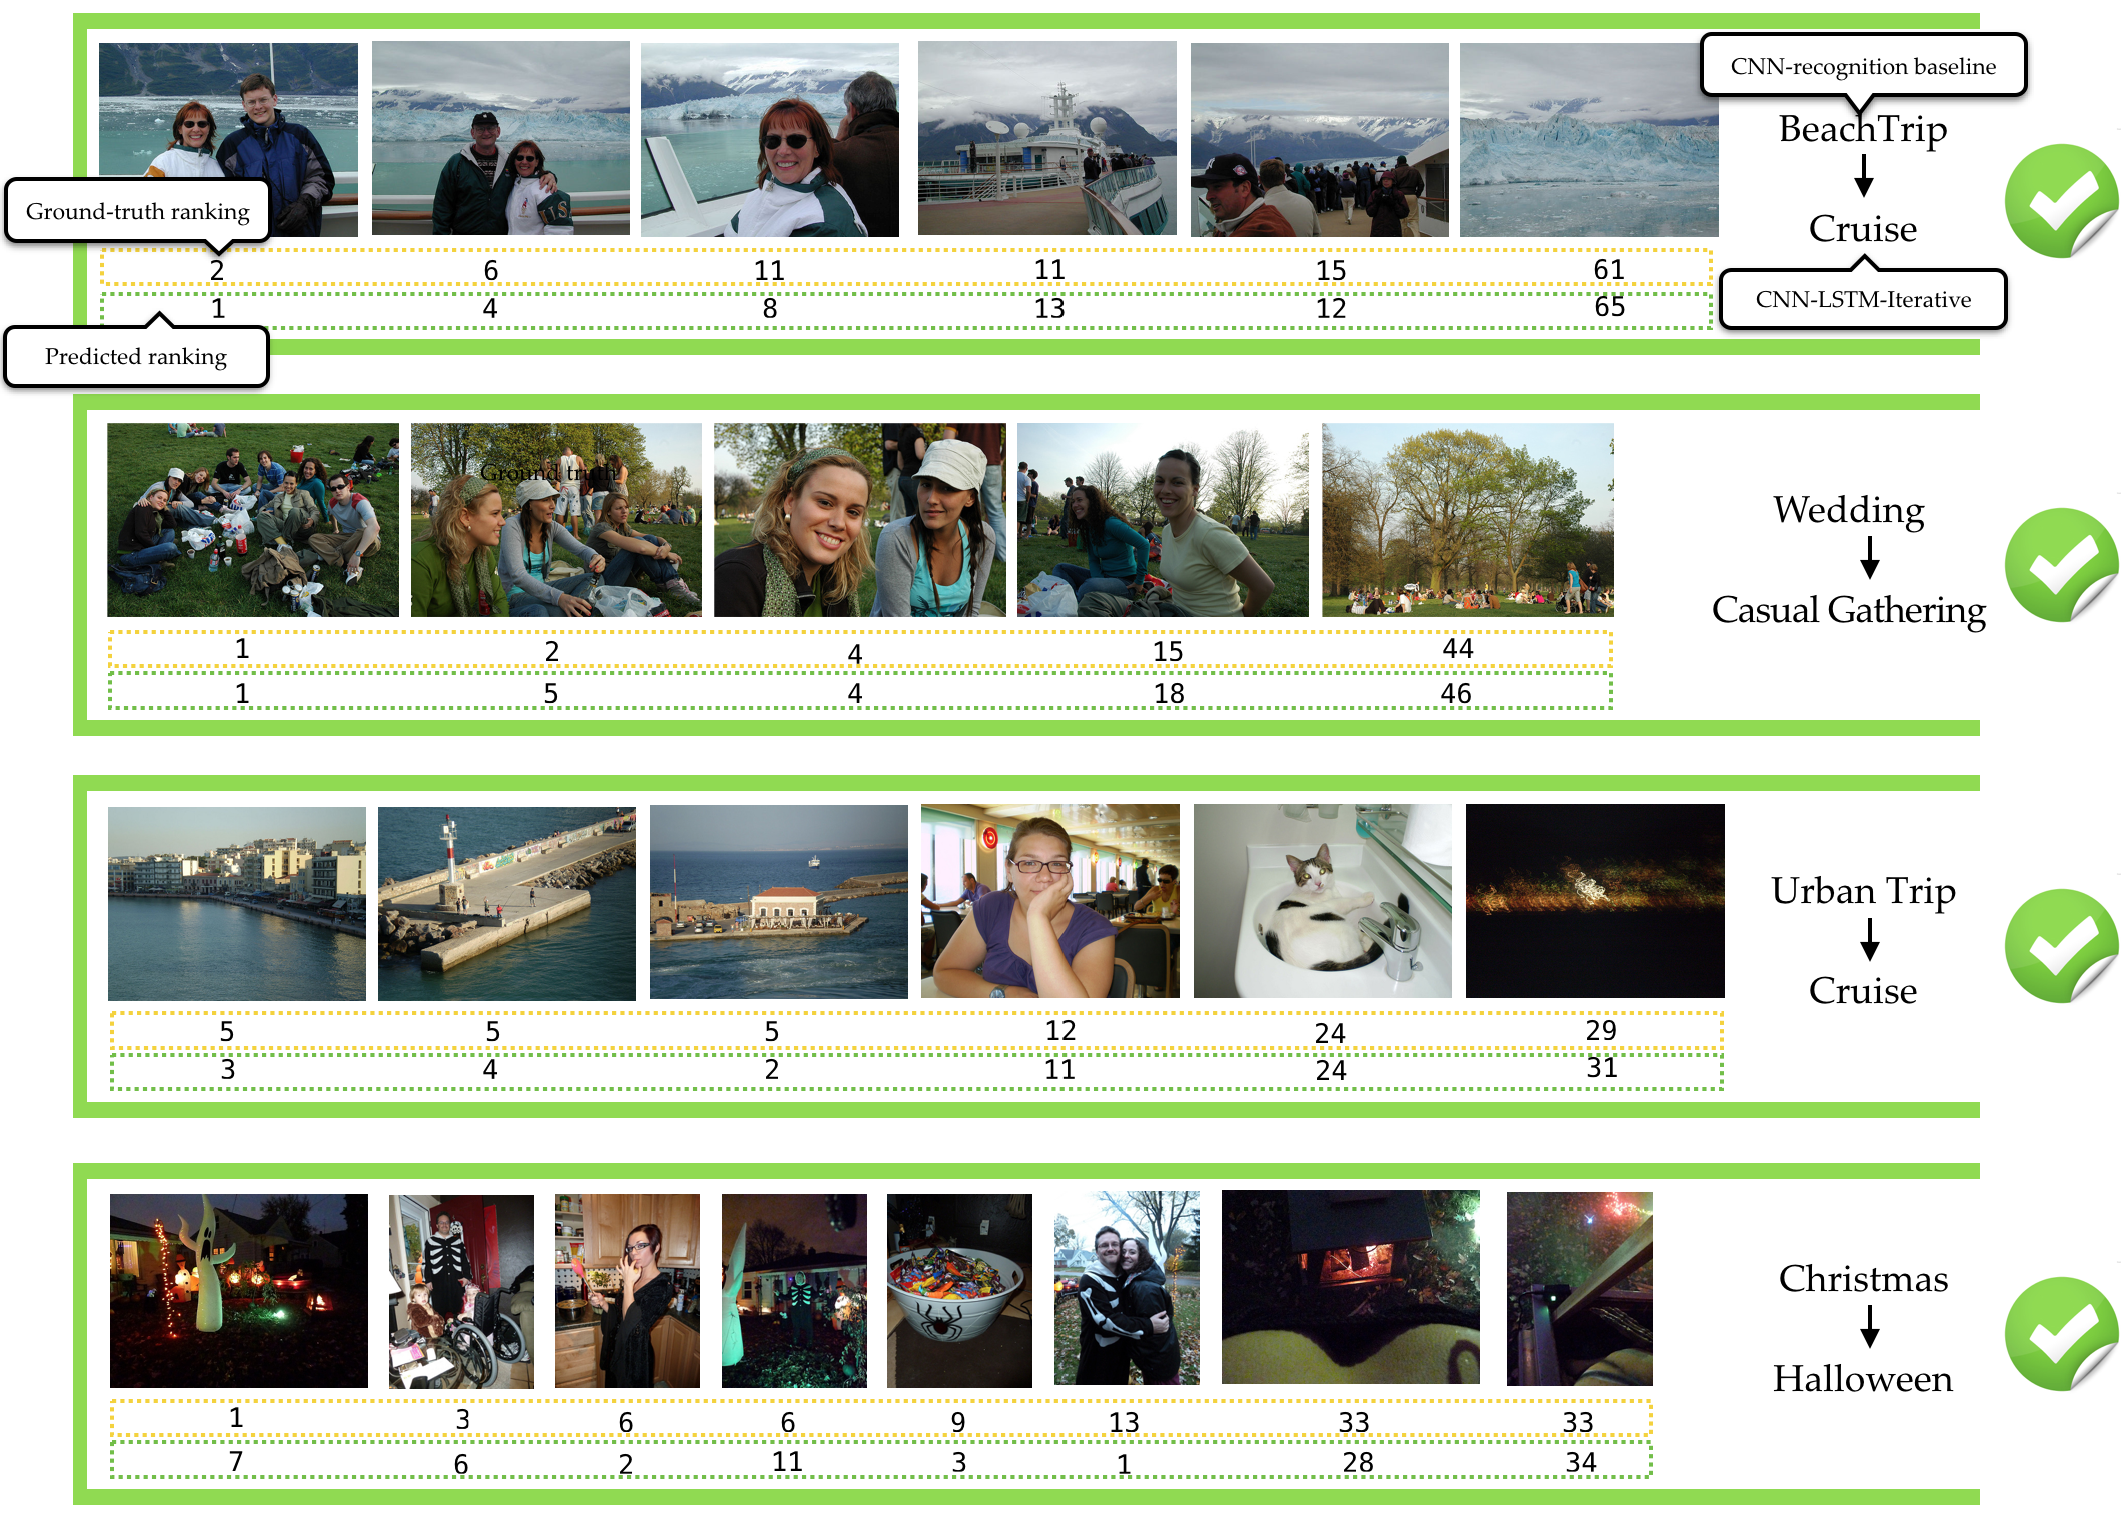
\includegraphics[width=5in]{correct1}
\caption{Examples of recognition-curation result from ML-CUFED Dataset.  These examples were incorrectly categorized by the CNN method, but correctly categorized by the CNN-LSTM network, as shown to the right of the album examples. Below the images, we show the ground-truth ranking of each image in the album and the predicted importance ranking of each image in the first and second row respectively.}
\label{correct1}
\vspace{-0.2in}
\end{figure}

In Figure~\ref{correct2}, more examples with correct event type prediction in ML-CUFED Dataset are shown. We can also see how the images are ranked with predicted importance by the algorithm.

\begin{figure}
\vspace{-0.1in}
\centering
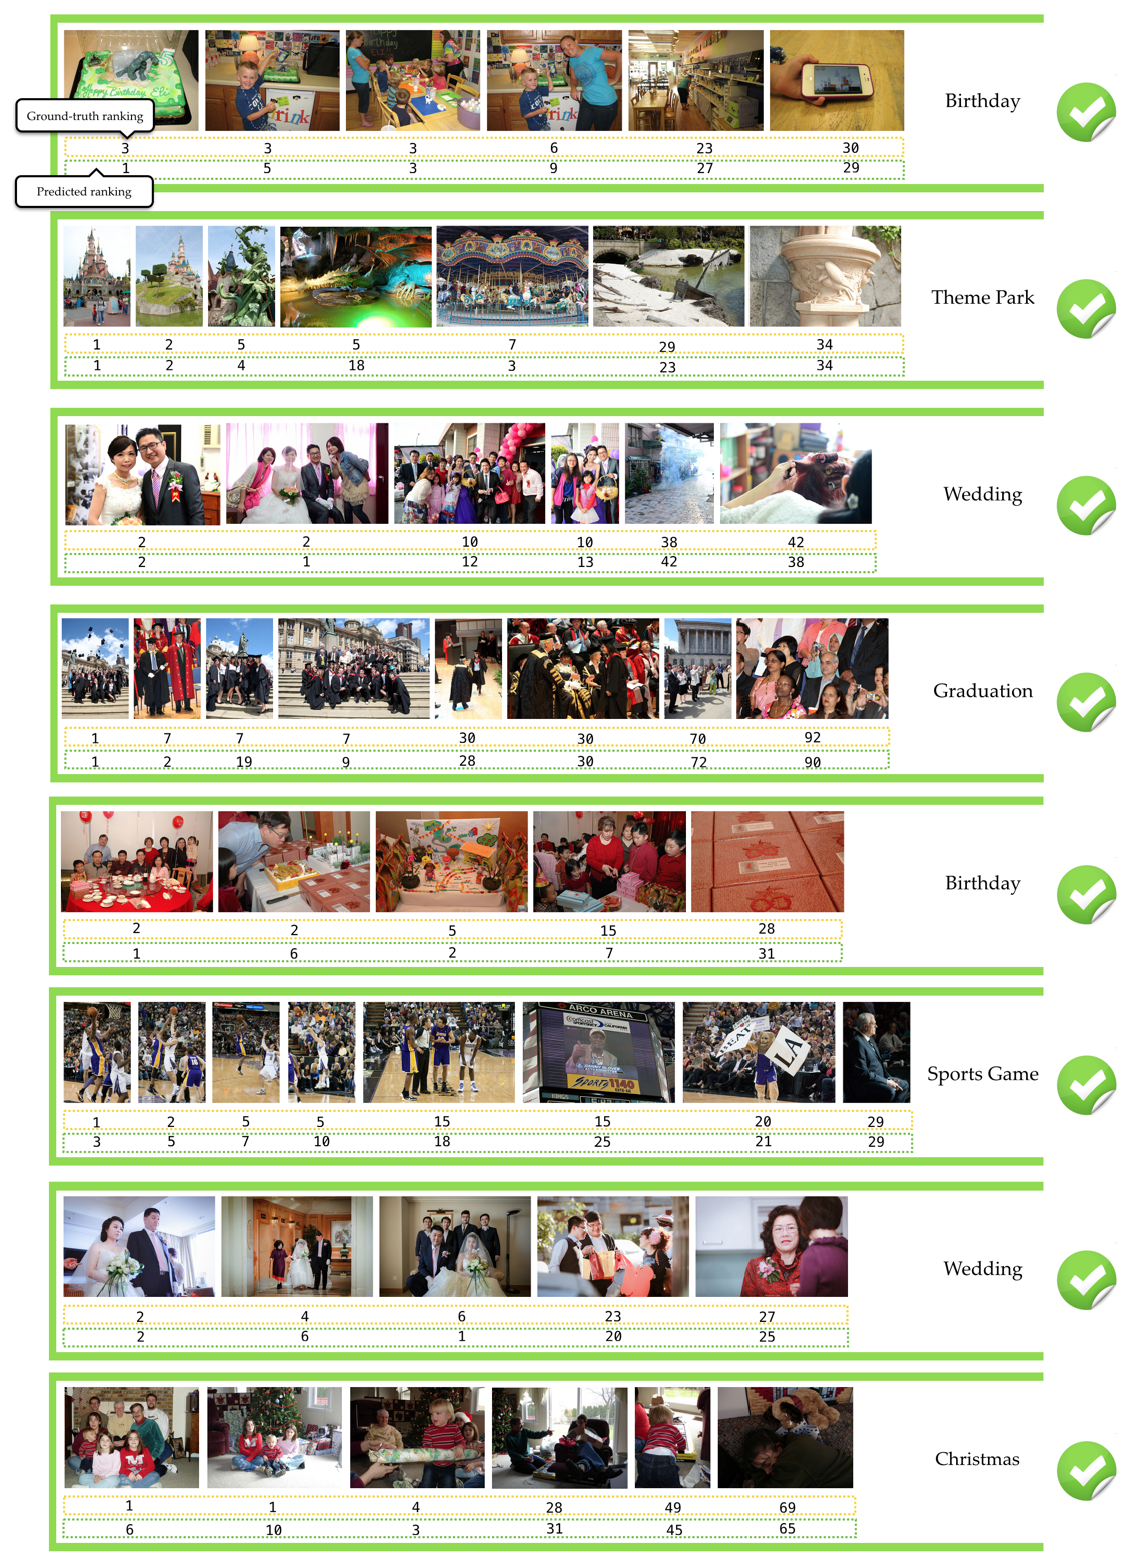
\includegraphics[width=5in]{correct2}
\caption{More examples of recognition-curation result from ML-CUFED Dataset. The event types of albums are correctly recognized, as shown in the right of each album.  Below each album, we show the ground-truth ranking and the predicted importance ranking for each image in the first and second row respectively.}
\label{correct2}
\vspace{-0.2in}
\end{figure}

In Figure~\ref{wrong1}, we show some examples with incorrect event type prediction in ML-CUFED Dataset. The ground-truth event type of the three example albums are book signing event, ball, and graduation party respectively.
\begin{figure}
\vspace{-0.1in}
\centering
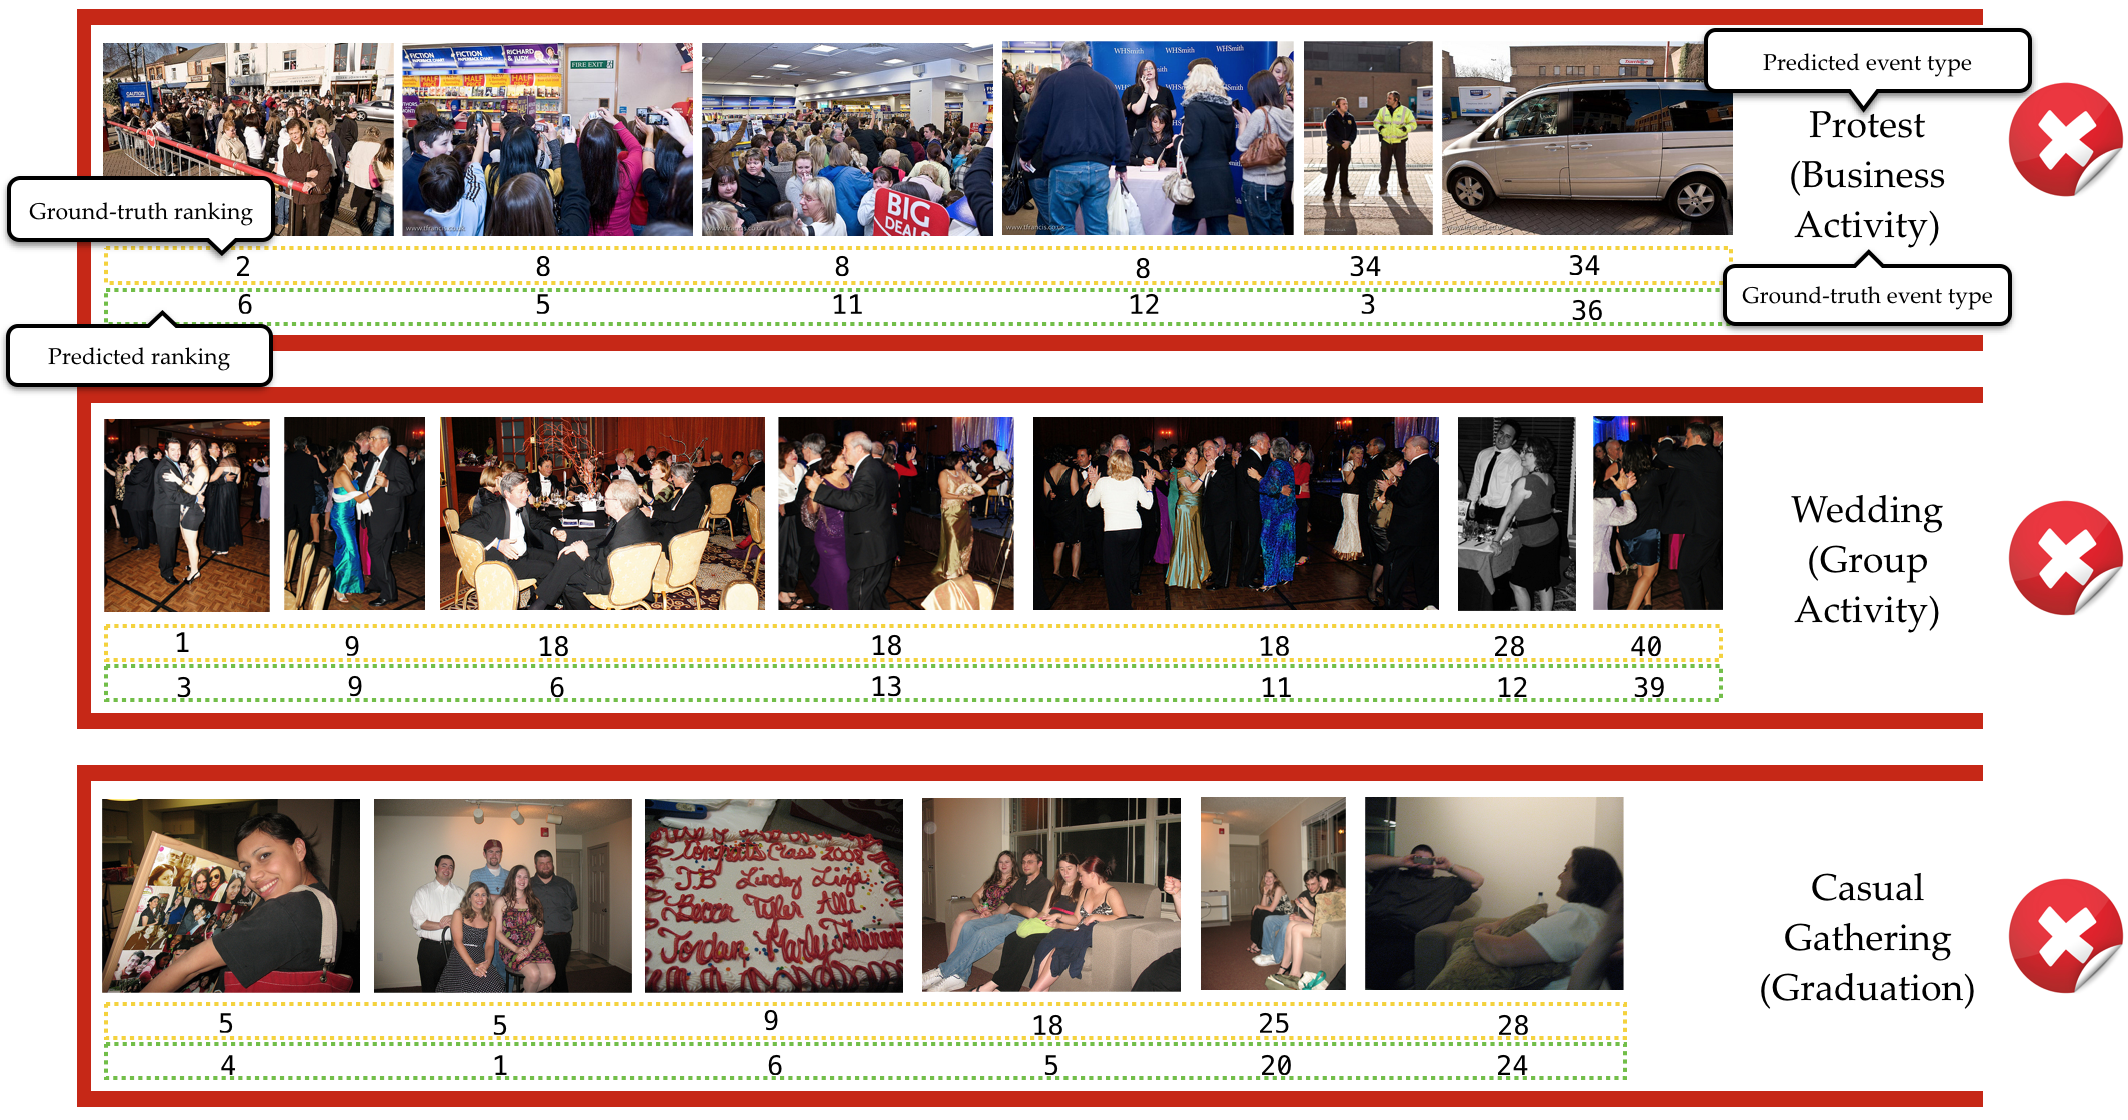
\includegraphics[width=5in]{wrong1}
\caption{Examples of recognition-curation result from ML-CUFED Dataset, whose event types are predicted incorrectly. The predicted event type and the ground-truth event type are shown in the right of each album. The ground-truth event type is shown in the parenthesis.}
\label{wrong1}
\vspace{-0.2in}
\end{figure}

\section{Long Short-Term Memory(LSTM) Network}
The architecture of the CNN-LSTM network for album-wise event type prediction is shown in Figure~\ref{LSTM}. The images of an album are first fed into the trained CNN for single images, and the 7th fully connected layer feature is extracted for each input image. The dimensionality of the FC7 features is then reduced to 128 with PCA, and the sequence of compressed features is fed into the LSTM network to predict the event type of the album for each time frame. The predictions are fed into a mean pooling layer for the final prediction.
\begin{figure}
\vspace{-0.1in}
\centering
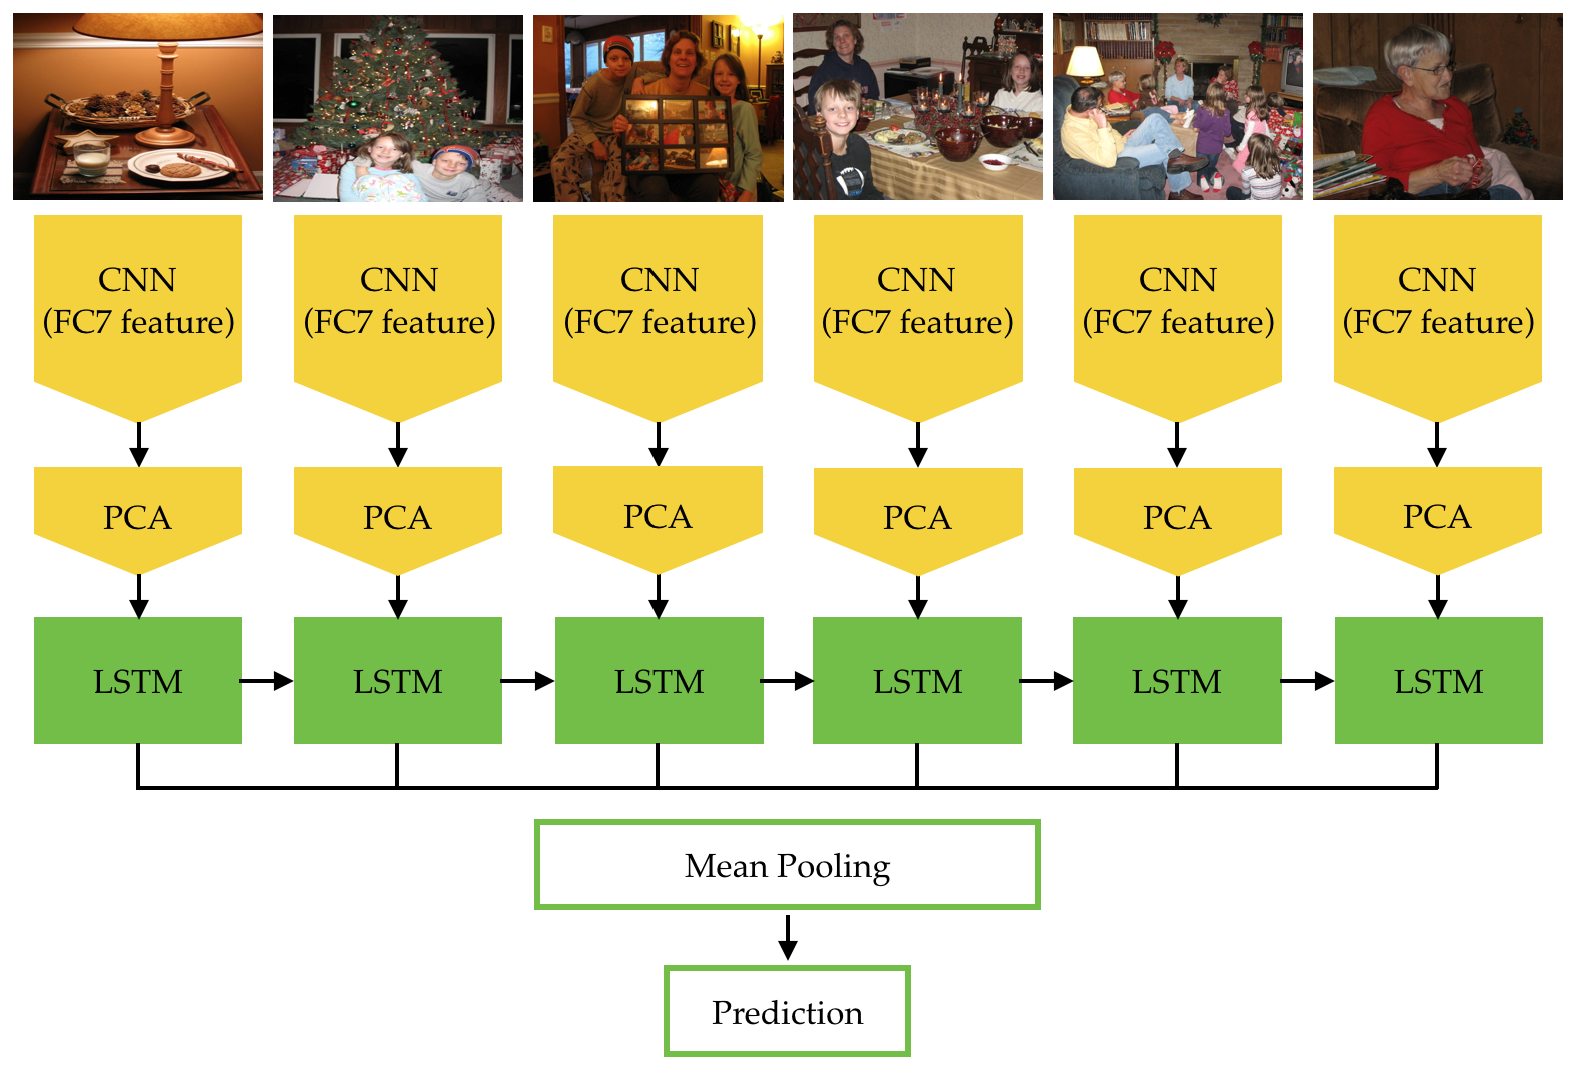
\includegraphics[width=4.5in]{LSTM}
\caption{Architecture of the CNN-LSTM network}
\label{LSTM}
\vspace{-0.2in}
\end{figure}

\bibliographystyle{splncs}
%\bibliography{egbib}
\end{document}
